\documentclass[12pt,a4paper,addpoints]{exam}

\usepackage[T1]{fontenc}
\usepackage{lmodern}
\usepackage{amsmath,amssymb,amsthm,mathtools}
\usepackage{bm}
\usepackage{booktabs}
\usepackage{graphicx}
\usepackage{xcolor}
\usepackage[shortlabels]{enumitem}
\usepackage{hyperref}
\usepackage[longnamesfirst]{natbib}
\bibliographystyle{ecta}

\renewcommand{\vec}{\bm}
\renewcommand{\phi}{\varphi}

\shadedsolutions
\definecolor{SolutionColor}{rgb}{0.9,0.95,1}
\renewcommand{\solutiontitle}{\noindent\emph{Solution} \par \noindent}

% Ignore any optional length argument on \begin{solution}[Xcm] — those
% annotations exist so the same source can be reused as a student exam
% (see exam.tex) where they become answer-box heights.
\cancelspacetrue

\newif\ifshowsolutions
\showsolutionsfalse % overridden by build script
\ifshowsolutions
\printanswers
\fi
\makeatletter
\qformat{%
    \thequestion. \bfseries\thequestiontitle
    \@ifundefined{pointsofq@\romannumeral\value{question}}{}{~(\totalpoints~points)}%
    \hfill}
\makeatother

\runningfooter{}{}{\copyright~Fabian Greimel, 2026}
\runningheader{{\sc Macroeconomics and Inequality}}{}{\thepage}

\title{Exercise Collection}
\author{Macroeconomics and Inequality}
\date{\today}

\begin{document}

\maketitle

\tableofcontents
\clearpage

\begin{questions}

\section{Elasticity of Intertemporal Substitution}
% !TeX root = ../exams/exam-2025.tex

\titledquestion{Elasticity of Intertemporal Substitution: Derivation}

\begin{parts}
    \part[3] Let $u$ be twice differentiable. Consider the function $f = {\ln} \circ {u'}$. (That is, $f(x) = \ln(u'(x))$.) Derive the linear approximation $\tilde f$ of $f$ around the point $x_0$.
    
    \begin{solution}[10.5cm]
        \begin{itemize}
            \item (1 point) General formula: $\tilde f(x) = f(x_0) + f'(x_0)(x - x_0)$
            \item (1 point) Derivative $({\ln} \circ {u'})'(x_0) = \frac{1}{u'(x_0)}\cdot u''(x_0)$
            \item (1 point) Solution $\tilde f(x) = \ln(u'(x_0)) + \frac{u''(x_0)}{u'(x_0)}(x - x_0)$
        \end{itemize}
    \end{solution}

    \part[1] Let $x_0 = c_j$. Compute $\tilde f(c_{j+1})$.

    \begin{solution}[7.5cm]
        $\tilde f(c_{j+1}) =  \ln(u'(c_j)) + \frac{u''(c_j)}{u'(c_j)}(c_{j+1} - c_j)$
    \end{solution}

    \part[4] Use (b) to show that
    \begin{equation*}
       \ln \biggl( \frac{u'(c_{j+1})}{u'(c_j)} \biggr) \approx \frac{c_{j+1} - c_j}{c_j} \frac{u''(c_j)}{u'(c_j)} c_j.
    \end{equation*}
   
    \begin{solution}[8cm]
        \begin{enumerate}
            \item (1.5 points) $f(c_{j+1}) \approx \tilde f(c_{j+1}) \implies  \ln(u'(c_{j+1})) \approx  \ln(u'(c_j)) + (c_{j+1} - c_j)\frac{u''(c_j)}{u'(c_j)}$
            \item (1.5 points) $\ln(a) - \ln(b) = \ln\bigl(\frac{a}{b}\bigr) \implies \ln\bigl(\frac{u'(c_{j+1})}{u'(c_j)}\bigr) \approx (c_{j+1} - c_j) \frac{u''(c_j)}{u'(c_j)}$
            \item (1 point) multiply $\frac{c_j}{c_j}$: $\ln\bigl(\frac{u'(c_{j+1})}{u'(c_j)}\bigr) \approx \frac{(c_{j+1} - c_j)}{c_j} \frac{u''(c_j)}{u'(c_j)} c_j$
        \end{enumerate}
    \end{solution}
    \part[4] Use the Euler equation $\beta (1+r) = \frac{u'(c_j)}{u'(c_{j+1})}$ and (c) to show that 
    \begin{equation*}
        \frac{d \frac{c_{j+1}- c_j}{c_j}}{d r} \approx  - \frac{u'(c_j)}{u''(c_j)c_j} 
    \end{equation*}
    \begin{solution}[8cm]
        \begin{enumerate}
            \item (1 point) Take logs $\ln(\beta (1+r)) = \ln\Bigl(\frac{u'(c_j)}{u'(c_{j+1})}\Bigr)$ 
            \item (1 point) Use $\ln(1+r) \approx r \implies \ln \beta + r \approx \ln\Bigl(\frac{u'(c_j)}{u'(c_{j+1})}\Bigr) = - \ln\Bigl(\frac{u'(c_{j+1})}{u'(c_j)}\Bigr)$ 
            \item (1 point) Use (c)
            \begin{align*}
                \ln \beta + r &\approx - \ln\Bigl(\frac{u'(c_{j+1})}{u'(c_j)}\Bigr) = - \frac{c_{j+1} - c_j}{c_j} \frac{u''(c_j)}{u'(c_j)} c_j \\
                \frac{c_{j+1} - c_j}{c_j} &\approx - \frac{u'(c_j)}{u''(c_j)c_j} \ln \beta + r
            \end{align*}
            \item (1 point) Take Derivative, done!
        \end{enumerate}
    \end{solution}
    \part[3] Interpret the expression in (d). 
    \begin{solution}[9cm]
        \begin{enumerate}
            \item (1 point) The right-hand side is the elasticity of intertemporal substitution.
            \item (2 points) It measures how does the steepness of the consumption profile (= growth rate of consumption) change when the interest rate (the relative price of consuming tomorrow) changes.
        \end{enumerate}
       
    \end{solution}
    \part[3] What is the sign of the elasticity of intertemporal substitution for concave $u$?
    \begin{solution}[9cm]
        \begin{enumerate}
            \item (1 point) Concave $u \implies u'' < 0$
            \item (1 point) We need the standard assumptions that $u' > 0$ and $c_j > 0$ 
            \item (1 point) Then $- \frac{u'(c_j)}{u''(c_j)c_j} > 0$.
        \end{enumerate} 
    \end{solution}
\end{parts}

\clearpage
\titledquestion{Elasticity of Intertemporal Substitution: Computation}

\begin{parts}
    \part[2] State the definition of the elasticity of intertemporal substitution.

    \begin{solution}[6cm]
        \begin{enumerate}
            \item (1 point) The EIS is the percentage response of the consumption growth rate $(c_{j+1} - c_j)/c_j$ to a percentage change in the gross interest rate (equivalently, the elasticity of the consumption ratio $c_{j+1}/c_j$ with respect to $1+r$).
            \item (1 point) Equivalently, for a smooth utility $u$,
            \begin{equation*}
                \text{EIS} = -\frac{u'(c)}{u''(c) \cdot c}.
            \end{equation*}
        \end{enumerate}
    \end{solution}

    \uplevel{From now on consider a household with utility function $u(c) = \frac{c^{1-\sigma}}{1-\sigma}$, $\sigma > 0$.}

    \part[4] Derive the elasticity of intertemporal substitution for that household.

    \begin{solution}[8cm]
        \begin{enumerate}
            \item (1 point) $u'(c) = c^{-\sigma}$
            \item (1 point) $u''(c) = -\sigma c^{-\sigma - 1}$
            \item (1 point) Substitute into $-\dfrac{u'(c)}{u''(c) \cdot c}$:
            \begin{equation*}
                -\frac{c^{-\sigma}}{-\sigma c^{-\sigma - 1} \cdot c} = \frac{c^{-\sigma}}{\sigma c^{-\sigma}}.
            \end{equation*}
            \item (1 point) Simplify: $\text{EIS} = \dfrac{1}{\sigma}$.
        \end{enumerate}
    \end{solution}

    \part[2] Discuss the role of the elasticity of intertemporal substitution in the Euler equation $\beta (1+r) = \frac{u'(c_j)}{u'(c_{j+1})}$.

    \begin{solution}[8cm]
        \begin{enumerate}
            \item (1 point) For CRRA utility the Euler equation becomes $\beta(1+r) = (c_{j+1}/c_j)^\sigma$. Taking logs and solving for consumption growth gives
            \begin{equation*}
                \ln\bigl(c_{j+1}/c_j\bigr) = \frac{1}{\sigma} \bigl[\ln \beta + \ln(1+r)\bigr] = \text{EIS} \cdot \bigl[\ln \beta + \ln(1+r)\bigr].
            \end{equation*}
            \item (1 point) The EIS is the slope of consumption growth with respect to $\ln(1+r)$. Households with a \emph{higher} EIS (smaller $\sigma$) readily substitute consumption across time, so their consumption profile tilts more steeply when the interest rate changes. Households with a \emph{lower} EIS (larger $\sigma$) prefer smooth consumption and respond less.
        \end{enumerate}
    \end{solution}
\end{parts}

\clearpage

\section{Household Decision Problems}
\input{../SimpleOLG/exercises/generated/mortality.tex}
\clearpage
\input{../SimpleOLG/exercises/generated/annuities.tex}
\clearpage
\input{../SimpleOLG/exercises/generated/bequests-warmglow-focs.tex}
\clearpage
\input{../SimpleOLG/exercises/generated/bequests-warmglow-solve.tex}
\clearpage
\input{../SimpleOLG/exercises/generated/entrepreneur-1period.tex}
\clearpage

% ---- Deferred exercises -------------------------------------------------
% Commented out for the initial student release. These exercises are sound
% in principle but need polish and consistency checks against the lecture
% notes before the final exam or next year's version:
%   - entrepreneur-2period (§2 Household Decision Problems)
%   - bequests-accidental, bequests-aggregation, bequests-equilibrium,
%     bequests-types (§3 OLG Aggregation and Stationary Equilibrium)
% olg-algorithm remains active so §3 still has one exercise.
% -------------------------------------------------------------------------
%\input{../SimpleOLG/exercises/generated/entrepreneur-2period.tex}
%\clearpage

\section{OLG Aggregation and Stationary Equilibrium}
%\input{../SimpleOLG/exercises/generated/bequests-accidental.tex}
%\clearpage
%\input{../SimpleOLG/exercises/generated/bequests-aggregation.tex}
%\clearpage
%\input{../SimpleOLG/exercises/generated/bequests-equilibrium.tex}
%\clearpage
%\input{../SimpleOLG/exercises/generated/bequests-types.tex}
%\clearpage
\input{../SimpleOLG/exercises/generated/olg-algorithm.tex}
\clearpage

\section{$J$-Period Lifecycle Problem}
% !TeX root = ../exams/exam-2025.tex

\titledquestion{Lifetime budget contraint}[7]

A household lives for $J = 4$ periods. The within-period budget constraint is given by

\begin{equation*}
    c_{j} + a_{j+1} = w \cdot y_{j} + a_j (1+r).
\end{equation*}

Derive the lifetime budget constraint of the household.

\begin{solution}[18cm]
    (1 point) Start with initial within-period budget constraint.
    \begin{align*}
        a_0 (1+r) &= c_{0} - w \cdot y_{0} + a_{1} \\
        \intertext{[1 point] Plug in for $a_1$}
                  &= c_{0} - w \cdot y_{0} + \frac{1}{1+r}(c_{1} - w \cdot y_{j} + a_{2})
        \intertext{[1 point] Plug in for $a_2$}
                  &= c_{0} - w \cdot y_{0} + \frac{1}{1+r}\Bigl((c_{1} - w \cdot y_{1} + \frac{1}{1+r}(c_{2} - w \cdot y_{2} + a_{3})\Bigr)
        \intertext{[1 point] Notice the pattern (note powers of 0 and 1)}
                  &= \Bigl(\frac{1}{1+r}\Bigr)^0(c_{0} - w \cdot y_{0}) + \Bigl(\frac{1}{1+r}\Bigr)^1(c_{1} - w \cdot y_{1}) + \Bigl(\frac{1}{1+r}\Bigr)^2(c_{2} - w \cdot y_{2}) + \Bigl(\frac{1}{1+r}\Bigr)^2 a_{3}
        \intertext{[1 point] Write in sum notation}
                  &= \sum_{j = 0}^3 \Bigl(\frac{1}{1+r}\Bigr)^j (c_j - w \cdot y_j) + \Bigl(\frac{1}{1+r}\Bigr)^3 a_4
        \intertext{[2 point] Write in canonical form; $0.5$ points for each correct term}
         &\implies \underbrace{\sum_{j = 0}^3 \Bigl(\frac{1}{1+r}\Bigr)^j c_j}_\text{consumption expenditures} + \underbrace{\Bigl(\frac{1}{1+r}\Bigr)^3 a_4}_\text{bequest} = \underbrace{\sum_{j = 0}^3 \Bigl(\frac{1}{1+r}\Bigr)^j (w \cdot y_j)}_\text{income} + \underbrace{a_0 (1+r)}_\text{inheritance}
    \end{align*}
\end{solution}
\clearpage
\titledquestion{$J$-period problem: Derivation}

A household lives for $J$ periods. The household maximizes

\begin{align*}
    & \max_{(c_j, a_{j+1})_j}\sum_{j=0}^{J-1} \beta^j u(c_j) \\
    & \begin{aligned}
        \text{subject to }
        & c_{j} + a_{j+1} = w \cdot y_{j} + a_j (1+r) \text{ for all $j \in \{0, \ldots, J-1$\}}, \\
        & a_J \geq 0, \\
        & a_0 = 0.
\end{aligned}
\end{align*}

\begin{parts}
    \part[3] State the household's lifetime budget constraint.

    \begin{solution}[14cm]
        \begin{align*}
            \intertext{[1 point] Use $a_0 = 0$; under positive marginal utility, $a_J = 0$ at the optimum.}
                a_{j+1} &= w \cdot y_j + (1+r) a_j - c_j
            \intertext{[1 point] Iterate forward from $j=0$:}
                0 = a_J &= \sum_{j=0}^{J-1} (1+r)^{J-1-j} (w y_j - c_j)
            \intertext{[1 point] Divide by $(1+r)^{J-1}$ to get the canonical form:}
                \sum_{j=0}^{J-1} \left(\frac{1}{1+r}\right)^{j} c_j &= \sum_{j=0}^{J-1} \left(\frac{1}{1+r}\right)^{j} w y_j.
        \end{align*}
    \end{solution}

    \part[2] What is the Lagrangian of this problem?

    \begin{solution}[5cm]
        \begin{align*}
            \intertext{[1 point] Objective:}
                \mathcal{L} &= \sum_{j=0}^{J-1} \beta^j u(c_j)
            \intertext{[1 point] add the multiplier on the lifetime budget constraint:}
                &\phantom{=} + \lambda \left[ \sum_{j=0}^{J-1} (1+r)^{-j} w y_j - \sum_{j=0}^{J-1} (1+r)^{-j} c_j \right].
        \end{align*}
    \end{solution}

    \part[2] What is the first-order condition with respect to $c_j$?

    \begin{solution}[5cm]
        \begin{align*}
            \intertext{[1 point] Differentiate $\mathcal{L}$ with respect to $c_j$:}
                \beta^j u'(c_j) - \lambda (1+r)^{-j} &= 0.
            \intertext{[1 point] Solve for $u'(c_j)$:}
                u'(c_j) &= \lambda \bigl[\beta (1+r)\bigr]^{-j}.
        \end{align*}
    \end{solution}

    \uplevel{From now on assume that $u(c) = \frac{c^{1-\sigma}}{1-\sigma}$, $\sigma > 0$.}

    \part[3] Write $c^*_j$ in terms of $c^*_{0}$.

    \begin{solution}[7cm]
        \begin{align*}
            \intertext{[1 point] Substitute $u'(c) = c^{-\sigma}$ into the FOC:}
                (c^*_j)^{-\sigma} &= \lambda \bigl[\beta (1+r)\bigr]^{-j}.
            \intertext{[1 point] Evaluate at $j=0$ to eliminate $\lambda$: $\lambda = (c^*_0)^{-\sigma}$. Divide the two:}
                \left(\frac{c^*_j}{c^*_0}\right)^{-\sigma} &= \bigl[\beta (1+r)\bigr]^{-j}.
            \intertext{[1 point] Solve for $c^*_j$:}
                c^*_j &= c^*_0 \bigl[\beta (1+r)\bigr]^{j/\sigma}.
        \end{align*}
    \end{solution}

    \part[2] Derive the Euler equation.

    \begin{solution}[6cm]
        \begin{align*}
            \intertext{[1 point] Take the ratio of the FOC at ages $j$ and $j+1$:}
                \frac{u'(c_j)}{u'(c_{j+1})} &= \frac{\lambda [\beta(1+r)]^{-j}}{\lambda [\beta(1+r)]^{-(j+1)}} = \beta(1+r).
            \intertext{[1 point] Rearrange:}
                u'(c_j) &= \beta (1+r) u'(c_{j+1}).
        \end{align*}
    \end{solution}

    \part[2] Interpret the Euler equation.

    \begin{solution}[7cm]
        \begin{itemize}
            \item [1 point] In the optimum the household is indifferent between consuming one unit today (marginal benefit $u'(c_j)$) and saving it to earn the gross return $1+r$, receiving $\beta(1+r)u'(c_{j+1})$ in discounted marginal utility tomorrow.
            \item [1 point] The sign of $\beta(1+r) - 1$ pins down the consumption profile: $\beta(1+r) > 1$ ($< 1$, $= 1$) yields an upward-sloping (downward-sloping, flat) path of consumption.
        \end{itemize}
    \end{solution}
\end{parts}

\clearpage
\input{../SimpleOLG/exercises/generated/dynamic-programming.tex}
\clearpage

%\section{EGM Implementation}
%\input{../SimpleOLG/exercises/generated/egm-credit-constraint.tex}
%\clearpage
%\input{../SimpleOLG/exercises/generated/egm-mortality-bequests.tex}
%\clearpage
%\input{../SimpleOLG/exercises/generated/egm-entrepreneur.tex}
%\clearpage

%\section{Social Comparisons}
%% !TeX root = ../collection-solutions.tex

\titledquestion{Social comparisons} In the model of \citet{drechsel2025falling-behind}, the optimal house of a given type~$i$
is given by $h^i = \kappa_2 y^i + \tilde \phi \tilde h^i$.

\begin{parts}

    \part Show that $\vec h = \kappa_2 (I + L) \vec y$ where $L$ is the social externality matrix.

    \begin{solution}
        \begin{itemize}
            \item Stack the equations: $\vec h = \kappa_2 \vec y + \tilde \phi \tilde{\vec h}$
            \item Use the definition $\tilde{\vec h} = G \vec h$: 
            $$\vec h = \kappa_2 \vec y + \tilde \phi G \vec h$$
            \item solve
            $$(I - \tilde \phi G)\vec h = \kappa_2 \vec y \implies \vec h = \kappa_2 (I - \tilde \phi G)^{-1} \vec y $$
            \item use that the Leontief inverse has a sum representation: $$(I - \tilde \phi G)^{-1} = \sum_{k=\textcolor{red}{0}}^\infty (\tilde \phi G)^k = I + \underbrace{\sum_{k=\textcolor{red}{1}}^\infty (\tilde \phi G)^k}_{=: L}$$
            \item Plug in: $\vec h = \kappa_2 (I + L) \vec y$
        \end{itemize}
    \end{solution}

    \part Compute $\frac{\partial}{\partial y^j} h^i$ (where $j \neq i$).

    \begin{solution}
        From (a) we know that $h_i = \kappa_2 (y_i + \sum_{\textcolor{blue}{k} = 1}^n  
        L_{i\textcolor{blue}{k}}
        y_{\textcolor{blue}{k}})
        $, where $L_{ik}$ is the $(i, k)$-entry of the social externality matrix $L$.

        Thus, $\frac{\partial}{\partial y^j} h^i = \kappa_2 L_{ij}$.
    \end{solution}

    \part Interpret this result and discuss its relevance.

    \begin{solution}
        \begin{itemize}
            \item   $L_{ij}$ is the externality that $j$ exerts on $i$. It is positive, if $\phi > 0$ and if $i$ cares about $j$'s house (directly or indirectly).

            \item If $j$'s income goes up, and $j$ exerts an externality on $i$, then $i$ will spend more on housing (and less on consumption).
    
            \item Such behavior is well-documented empirically. It can help explain why household debt has increased so much between 1980 and 2007.  
        \end{itemize}
      \end{solution}

\end{parts}
%\clearpage
%% !TeX root = ../collection-solutions.tex

% Comparisons 2
\titledquestion{Social comparisons} Consider the model of social comparisons by \citet{drechsel2025falling-behind}
with three types ($P$, $M$, $R$), weights $\vec \omega = (\omega_P, \omega_M, \omega_R)$ 
and 
%XXXXX
some comparison network $G$.

    Consider a \emph{low inequality} steady state 
    with incomes $\underline{\vec y} = (\underline y^P, \underline y^M, \underline y^R)$
    and a \emph{high inequality} steady state 
    with incomes $\overline{\vec y} = (\overline y^P, \overline y^M, \overline y^R)$.
    
    In the \emph{high inequality} steady state $R$ is richer, and $P$ is poorer than in the \emph{low inequality} state:%
    %
    \begin{equation*}
        \omega_R \Delta y^R = - \omega_P \Delta y^P > 0, \quad \text{and } \Delta y^M = 0.
    \end{equation*}
    where $\Delta y^i = \overline y^i - \underline y^i$.
    
    Recall that aggregate debt can be written as $D(\vec y) = \kappa_3 (\vec \omega + \vec b)^T \vec y$, where $\vec b$ is the vector of popularities.

    \begin{parts}
        \part Derive the condition, under which debt is higher in the \emph{high inequality steady state}: $D(\overline{ \vec y}) > D(\underline{\vec y})$

        \begin{solution}
            \begin{enumerate}
                \item Note that $$(\overline{ \vec y}) > D(\underline{\vec y}) \iff D(\overline{ \vec y}) - D(\underline{\vec y}) = \textcolor{gray}{\kappa_3} \sum_{i = 1}^n (\omega_i + b_i) \Delta y^i  > 0$$
                \item This sum has only two positive entries, because only $y^P, y^R \neq 0$. Hence
                $$\iff (\omega_P + b_P) \Delta y^P + (\omega_R + b_R) \Delta y^R  > 0$$
            
                \item Use that $\Delta y^R = - \frac{\omega_P}{\omega_R} \Delta y^P$. Then
                $$ (\omega_P + b_P) \Delta y^P - (\omega_R + b_R) \frac{\omega_P}{\omega_R}\Delta y^P  > 0 $$

                (or, alternatively, $ -(\omega_P + b_P) \frac{\omega_R}{\omega_P}\Delta y^R + (\omega_R + b_R) \Delta y^R  > 0 $)

                \item This simplifies to
                
                $$D(\overline{ \vec y}) > D(\underline{\vec y}) \iff \frac{b_P}{\omega_P} < \frac{b_R}{\omega_R}.$$

                (Note that $\Delta y^P < 0 < \Delta y^R$!)
            \end{enumerate}
        \end{solution}

        \part Interpret this result and discuss its relevance.

        \begin{solution}
            \begin{itemize}
                \item Income inequality has been rising in the past decades: The income share of the bottom 50\% has fallen, while the income share of the top 10\% has increased. 

                \item Empirically, social comparisons tend to be upward looking, that means that $R$ is more popular than $P$. Thus the condition $\frac{b_P}{\omega_P} < \frac{b_R}{\omega_R}$ is satisfied.
    
                \item This model predicts that increasing inequality \emph{causes} a rise in household debt. 
                
                \item Consistent with this, the data show that there is a positive \emph{correlation} between debt and inequality.
            \end{itemize}
        \end{solution}
    \end{parts}
%\clearpage
%% !TeX root = ../collection-solutions.tex

% Comparisons 3
\titledquestion{Social comparisons} Consider the model of social comparisons by \citet{drechsel2025falling-behind} 
    with three types ($P$, $M$, $R$), weights $\vec \omega = (\omega_P, \omega_M, \omega_R)$ 
    and the following comparison network $G$.

    \begin{center}
        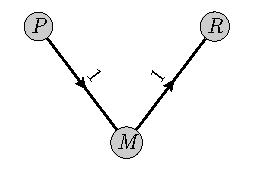
\includegraphics{comparisons/comparison-network-richer}
    \end{center}

    \begin{parts}
        \part Let $\tilde \phi = \kappa_1 \phi$. Compute the social externality matrix $L$.

        \begin{solution}
        
            $G = \begin{pmatrix}
                0 & 1 & 0 \\ 0 & 0 & 1 \\ 0 & 0 & 0
            \end{pmatrix}$, 
            %
            $G^2 = \begin{pmatrix}
                0 & 0 & 1 \\ 0 & 0 & 0 \\ 0 & 0 & 0
            \end{pmatrix}$,
            %
            $G^3 = G^4 = \cdots = 0 \in \mathbb{R}^{3 \times 3}$

            Hence,

            $L = \sum_{i=1}^\infty \phi^i G^i = \begin{pmatrix}
                0 & \tilde \phi & \tilde \phi^2 \\
                 0 & 0 & \tilde \phi \\ 
                 0 & 0 & 0 \\
            \end{pmatrix}$
        \end{solution}

        \uplevel{Consider a \emph{low inequality} steady state 
        with incomes $\underline{\vec y} = (\underline y^P, \underline y^M, \underline y^R)$
        and a \emph{high inequality} steady state 
        with incomes $\overline{\vec y} = (\overline y^P, \overline y^M, \overline y^R)$.
        
        In the \emph{high inequality} steady state $R$ is richer, and $P$ is poorer than in the \emph{low inequality} state:%
        %
        \begin{equation*}
            \omega_R \Delta y^R = - \omega_P \Delta y^P > 0, \quad \text{and } \Delta y^M = 0.
        \end{equation*}
        where $\Delta y^i = \overline y^i - \underline y^i$.
        }
        \part Will aggregate debt $D$ be higher or lower in the high inequality steady state? \emph{Use the relevant result from Drechsel-Grau and Greimel (2024).}

        \begin{solution}
            The relevant condition is  $$D(\overline{ \vec y}) > D(\underline{\vec y}) \iff \frac{b_P}{\omega_P} < \frac{b_R}{\omega_R}.$$

            Note that $b_P = 0$ and $b_R = \omega_M \tilde \phi + \omega_P \tilde \phi^2 > 0$. Hence the above condition is satisfied (higher debt in \emph{high inequality} steady state).
        \end{solution}
       
        \part Interpret this result and discuss its relevance.

        \begin{solution}
            \begin{itemize}
                \item Income inequality has been rising in the past decades: The income share of the bottom 50\% has fallen, while the income share of the top 10\% has increased. So we can interpret the two steady states corresponding to some decades age (e.g.\ 1980) vs now.

                \item Empirically, social comparisons tend to be upward looking, so the given $G$ might be a good approximation of reality.
    
                \item This model predicts that increasing inequality \emph{causes} a rise in household debt.
                
                \item Consistent with this, the data show that there is a positive \emph{correlation} between debt and inequality.
            \end{itemize}
        \end{solution}
    \end{parts}
%\clearpage
%\input{comparisons/comparisons4-mean.tex}
%\clearpage
%% !TeX root = ../collection-solutions.tex

% Comparisons 4
\titledquestion{Social comparisons} Consider the model of social comparisons by \citet{drechsel2025falling-behind}
with three types ($P$, $M$, $R$), weights $\vec \omega = (\omega_P, \omega_M, \omega_R)$ 
and the following comparison network $G$.%

    \begin{center}
        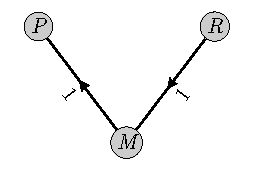
\includegraphics{comparisons/comparison-network-poorer}
    \end{center}

    \begin{parts}
        \part Let $\tilde \phi = \kappa_1 \phi$. Compute the social externality matrix $L$.

        \begin{solution}
        
            $G = \begin{pmatrix}
                0 & 0 & 0 \\ 1 & 0 & 0 \\ 0 & 1 & 0
            \end{pmatrix}$, 
            %
            $G^2 = \begin{pmatrix}
                0 & 0 & 0 \\ 0 & 0 & 0 \\ 1 & 0 & 0
            \end{pmatrix}$,
            %
            $G^3 = G^4 = \cdots = 0 \in \mathbb{R}^{3 \times 3}$

            Hence,

            $L = \sum_{i=1}^\infty \phi^i G^i = \begin{pmatrix}
                0 & 0 & 0 \\ \tilde \phi & 0 & 0 \\ \tilde \phi^2 & \tilde \phi & 0
            \end{pmatrix}$
        \end{solution}
        
        \uplevel{Recall that $\vec h = \kappa_2 \sum_{i = 0}^\infty (\tilde \phi G)^i \vec y$.}

        \part Compute $\frac{\partial}{\partial y^R} h_P$.

        \begin{solution}
            \begin{itemize}
                \item Note that $\sum_{i = 0}^\infty (\tilde \phi G)^i = I + L$
                \item Thus $\frac{\partial}{\partial y^R} h_P = \kappa_2 L_{PR}$ where $L_{PR}$ is the $(P, R)$ entry of the social externality matrix $L$.
                \item $L_{PR} = 0$ (from above)
            \end{itemize}
        \end{solution}

        \part Interpret this result and discuss its relevance.

        \begin{solution}
            \begin{itemize}
                \item $L_{ij}$ is the externality that $j$ exerts on $i$. It is positive, if $\phi > 0$ and if $i$ cares about $j$'s house (directly or indirectly).

                \item If $j$'s income goes up, and $j$ exerts an externality on $i$, then $i$ will spend more on housing (and less on consumption).
        
                \item Such behavior is well-documented empirically. It can help explain why household debt has increased so much between 1980 and 2007.
            \end{itemize}
        \end{solution}
    \end{parts}

\clearpage
% The "Required Reading" section: exercises paired with the reading assignments.
% This file is \input inside collection.tex's top-level questions environment,
% so it must NOT open its own questions environment (the exercises-repo original
% did; this public copy deliberately drops that wrapper and the \section name).

\section{Required Reading}

% Paired paper exercises: question n' repeats the previous number with a prime.
\newcommand{\primedquestion}{\addtocounter{question}{-1}\renewcommand{\thequestion}{\arabic{question}$'$}}
\newcommand{\unprimedquestion}{\renewcommand{\thequestion}{\arabic{question}}}

Like the reading assignments, the exercises in this section come in pairs:
exercises $n$ and $n'$ cover the two papers of one assignment pair. Answer the
questions for the paper that you have read. The wealth-tax contrast exercise can
be answered with either paper of its pair.

% !TeX root = ../collection-solutions.tex

\titledquestion{Sources of US wealth inequality}

\citet{hubmer2021sources} ask which forces account for the rise in US top wealth shares since the 1960s.

\begin{parts}
    \part[4] What is the key takeaway of the paper? Explain how the authors arrive at this conclusion: what kind of model do they use, what disciplines it, and what is the experiment behind the headline result?

    \begin{solutionorbox}[12cm]
        \emph{Takeaway} (2 points): Two complementary results — one about the \emph{level}, one about the \emph{change}. (i)~Return heterogeneity is needed to match the \emph{level} of US wealth concentration: with portfolio returns whose mean and risk rise with wealth, the model reproduces the 1967 distribution, including its thick top tail (steady-state decomposition). (ii)~The decline in US tax progressivity is by far the largest driver of the \emph{rise} in top wealth shares since the 1960s (dynamic decomposition) — return heterogeneity is the engine that makes the wealthy able to pull away, and falling progressivity is what unleashed it. Side results: rising \emph{earnings risk} actually \emph{reduces} top wealth shares, and movements in asset-class return premia explain the medium-run U-shape of top shares but contribute negatively on net over the whole period.

        \emph{How they get there} (2 points):
        \begin{itemize}
            \item A standard incomplete-markets (Aiyagari-style) model extended with \emph{wealth-dependent return heterogeneity}: both the mean and the idiosyncratic risk of portfolio returns rise with wealth. These return schedules are disciplined by administrative portfolio data (rather than calibrated to wealth moments), which lets the model match the 1967 US wealth distribution — including the thick top tail — as a steady state.
            \item The model is then fed the observed historical \emph{paths} of (i) effective tax schedules, (ii) top earnings inequality, (iii) earnings risk, and (iv) asset-class return premia, and the implied transition 1967--2012 is compared with the data: the model reproduces most of the observed rise in the top 1\% share.
            \item Decomposition: feeding in one channel at a time shows taxes account for (more than) the entire explained rise, top earnings inequality for a small positive part, while earnings risk and return premia contribute \emph{negatively}.
        \end{itemize}
        Grading: 1 point for the level result (return heterogeneity matches the 1967 distribution), 1 point for the change result (declining tax progressivity drives the rise); 1 point for model + data discipline of the return schedules, 1 point for the feed-in-historical-paths / one-channel-at-a-time experiment. Mentioning a counterintuitive side result (earnings risk negative; return premia generate the U-shape) can substitute for one of the first two points.
    \end{solutionorbox}

    \part[4] Explain intuitively why a \emph{less progressive} tax system increases top wealth concentration so powerfully in this model. Your answer should explain how the model generates a thick upper tail of the wealth distribution, and how tax progressivity interacts with that force.

    \begin{solutionorbox}[12cm]
        \begin{itemize}
            \item (2 points) \emph{Where the thick tail comes from:} for rich, well-insured households, saving is approximately proportional to wealth, with a random coefficient — wealth grows multiplicatively at a stochastic rate determined by the (heterogeneous, risky) portfolio return. Random multiplicative growth of this kind generates a Pareto upper tail, and the thickness of the tail increases with the \emph{dispersion} of after-tax returns.
            \item (1 point) \emph{What progressivity does:} a progressive tax compresses \emph{after-tax} returns and resources across households — the rich face persistently higher marginal rates. This acts exactly like a reduction in return dispersion: it is the glue that keeps the top of the distribution together.
            \item (1 point) \emph{Hence the result:} cutting progressivity removes that glue. After-tax returns and the resources available for saving fan out again, the saving propensities of the richest rise relative to everyone else's, and the Pareto tail thickens — top wealth shares rise strongly. (Bonus insight: the same logic explains why \emph{more} earnings risk lowers top shares — precautionary saving compresses the bottom and, in general equilibrium, depresses the interest rate and thins the tail.)
        \end{itemize}
    \end{solutionorbox}
\end{parts}

\primedquestion
% !TeX root = ../collection-solutions.tex

\titledquestion{Why are the wealthiest so wealthy?}

\citet{hubmer2026wealthiest} use Norwegian administrative panel data to trace how the top 0.1\% accumulated their wealth over 26 years.

\begin{parts}
    \part[4] What is the key takeaway of the paper? Explain how the authors arrive at this conclusion: what is the decomposition method, what are the headline magnitudes, and how do the authors use these facts to discriminate between theories of wealth inequality?

    \begin{solutionorbox}[12cm]
        \emph{Takeaway} (2 points): The excess wealth of the top 0.1\% over the median household is accounted for by higher \emph{saving rates} ($\approx 36\%$), \emph{inheritances} ($\approx 31\%$), higher \emph{returns} ($\approx 28\%$) and higher labor income ($\approx 5\%$). These \emph{dynamic} facts reject all standard single-channel models of wealth inequality — even though each of them (suitably augmented) can match the cross-sectional concentration of wealth. Only a model combining entrepreneurship with decreasing returns to scale and non-homothetic (``capitalist spirit'') saving preferences fits the dynamics.

        \emph{How they get there} (2 points):
        \begin{itemize}
            \item Method: track households backward over 26 years through their \emph{budget identity} (wealth growth $=$ returns $+$ labor income $+$ inheritances, scaled by the saving rate). Replace one component at a time with the value of the middle class and recompute the counterfactual wealth path; average over all replacement orderings (Shapley--Owen) so the contributions sum to 100\%. This is an \emph{accounting} decomposition — it deliberately holds behavior fixed.
            \item A quarter of the top 0.1\% are ``New Money'': they start with roughly zero (on average negative) wealth and rise on extremely high returns and saving rates; ``Old Money'' heirs grow already-large fortunes mainly through inheritances and persistently high saving, with only modest returns.
            \item Model horse race: standard models (superstar earnings, heterogeneous returns, discount-factor heterogeneity, bequest motives) are each recalibrated to match cross-sectional wealth concentration, then confronted with the decomposition. Each fails in a characteristic way — e.g.\ the bequest and return-heterogeneity models attribute far too much to inheritances, the superstar model far too much to labor income and produces no Old Money.
        \end{itemize}
        Grading: 1 point for the four shares (approximate), 1 point for ``dynamics reject models that match the cross-section''; 1 point for the budget-identity/counterfactual-replacement method (incl.\ its accounting nature), 1 point for New vs.\ Old Money or a concrete model failure.
    \end{solutionorbox}

    \part[4] The data demand two things at once: self-made households that reach the top 0.1\% within $\sim$25 years (``New Money''), and heirs who keep growing large fortunes at high saving rates but moderate returns (``Old Money''). Explain intuitively how (i) entrepreneurship with decreasing returns to scale and a collateral constraint and (ii) non-homothetic ``capitalist spirit'' preferences jointly deliver both.

    \begin{solutionorbox}[12cm]
        \begin{itemize}
            \item (2 points) \emph{Decreasing returns + collateral constraint make returns non-monotone in wealth.} Across households, productivity and wealth are positively correlated, so \emph{average} returns rise with wealth (as in the data). But for a \emph{given} entrepreneur, the marginal return falls as the firm grows. A young, highly productive but collateral-constrained entrepreneur earns very high returns on a small base — the New Money rocket — while the same decreasing returns cap returns once the firm matures, so fortunes do not diverge without bound and established wealth earns only moderate returns (as Old Money does).
            \item (1 point) \emph{Non-homothetic preferences keep rich households saving.} With wealth in the utility function, the saving rate \emph{rises} with resources, so rich households — including heirs whose returns are unspectacular — keep saving large fractions of their income throughout life. This is what generates Old Money's high saving contribution, which returns alone cannot explain.
            \item (1 point) \emph{Timing matters:} unlike a warm-glow bequest motive, which only becomes relevant near the end of life (it is weighted by the probability of dying), the capitalist-spirit motive operates from the start — so \emph{young} wealthy households already save at high rates, as in the data. In a pure bequest model, young heirs would instead run down their wealth first.
        \end{itemize}
    \end{solutionorbox}
\end{parts}

\unprimedquestion
% !TeX root = ../collection-solutions.tex

\titledquestion{Use it or lose it: taxing wealth instead of capital income}

\citet{guvenen2023use} study what happens when the United States replaces its capital income tax with a flat tax on wealth.

\begin{parts}
    \part[4] What is the key takeaway of the paper? Explain how the authors arrive at this conclusion: what kind of model do they use, how is it disciplined by data, and what is the main quantitative experiment behind the headline result?

    \begin{solutionorbox}[12cm]
        \emph{Takeaway} (2 points): When returns to wealth differ persistently across people, taxing wealth and taxing capital income are no longer equivalent. Replacing the US capital income tax with a revenue-neutral flat wealth tax raises output, wages and welfare (newborn welfare gain of $\approx 7\%$ in consumption-equivalent terms, with about two thirds of the population gaining). The optimal wealth tax is high ($\approx 3\%$), while the optimal capital \emph{income} tax would be a subsidy.

        \emph{How they get there} (2 points):
        \begin{itemize}
            \item A quantitative overlapping-generations model in which entrepreneurs differ in productivity (rate of return) and face collateral constraints, so wealth is not automatically allocated to its most productive use.
            \item The calibration matches US wealth concentration (top 1\% wealth share, Pareto tail, share of self-made billionaires); the model also reproduces the dispersion and persistence of returns measured in Norwegian administrative data \emph{without targeting them}.
            \item Main experiment: a revenue-neutral tax swap (capital income tax out, flat wealth tax of $\approx 1.2\%$ in). Capital rises by $\approx 16\%$, aggregate TFP by $\approx 2\%$, wages by $\approx 8\%$ — and most of the welfare gain comes through higher wages, which is why gains are broad-based even though wealth inequality \emph{rises}.
        \end{itemize}
        Grading: 1 point for the non-equivalence/efficiency-ranking insight, 1 point for the headline welfare result; 1 point for model + calibration, 1 point for the experiment with (approximate) magnitudes and the wage channel.
    \end{solutionorbox}

    \part[4] A common intuition is that a wealth tax punishes saving and should therefore shrink the economy. Explain intuitively the \emph{use-it-or-lose-it} mechanism by which the wealth tax raises productivity in this model.

    \begin{solutionorbox}[12cm]
        \begin{itemize}
            \item (1 point) A capital income tax is paid only on income \emph{generated}: productive entrepreneurs bear the entire burden, while idle wealth escapes taxation. A wealth tax is paid on the \emph{stock}: two people with the same wealth pay the same tax regardless of how productively they use it.
            \item (1 point) Switching to the wealth tax therefore broadens the tax base and shifts the burden from high-return to low-return wealth holders: ``use it or lose it''.
            \item (1 point) Because after-tax return \emph{differences} are preserved (rather than compressed by the income tax), behavior responds: high-return entrepreneurs save more, low-return holders run down their wealth. With collateral constraints, the wealth shed by unproductive holders is lent to productive but constrained entrepreneurs.
            \item (1 point) The same aggregate capital stock then produces more output: TFP rises, labor demand and wages rise, so the gains accrue broadly — even though wealth concentration at the top increases.
        \end{itemize}
    \end{solutionorbox}
\end{parts}

\primedquestion
% !TeX root = ../collection-solutions.tex

\titledquestion{Should we tax capital income or wealth?}

\citet{boar2023income-or-wealth} ask which asset-side tax instrument a welfare-maximizing planner should use: a tax on capital income or a tax on wealth.

\begin{parts}
    \part[4] What is the key takeaway of the paper? Explain how the authors arrive at this conclusion: what kind of model do they use, which features of the US data does the calibration target, and why does this calibration matter for the result?

    \begin{solutionorbox}[12cm]
        \emph{Takeaway} (2 points): Taxing capital income beats taxing wealth. A utilitarian planner restricted to one instrument achieves a consumption-equivalent welfare gain of $\approx 9.5\%$ with a (high) capital income tax but only $\approx 5.6\%$ with a wealth tax — and when both instruments are available, the optimal wealth tax is \emph{zero}. The efficiency gains from wealth taxation are real but small, and are swamped by the redistributive power of taxing entrepreneurs' profits.

        \emph{How they get there} (2 points):
        \begin{itemize}
            \item A general-equilibrium model with entrepreneurs facing collateral constraints (as in Guvenen et al.) — but alongside an \emph{unconstrained corporate sector}, and with entrepreneurial technology that uses labor and has decreasing returns.
            \item The calibration targets how much of US wealth and income private business owners actually hold (SCF: entrepreneurs are $\approx 12\%$ of households but hold $44\%$ of wealth and $28\%$ of income). In the calibrated economy, misallocation losses are only $\approx 1.3\%$ of output — capital that constrained entrepreneurs cannot absorb flows to the unconstrained corporate sector, and persistently productive entrepreneurs save their way out of their constraints.
            \item Optimal-policy experiment: one-time permanent tax reforms, with welfare computed \emph{including the transition} and revenue rebated as lump-sum transfers. Because the efficiency pie is tiny while the redistribution stakes are large, the instrument that targets rich entrepreneurs' profits (the capital income tax) wins.
        \end{itemize}
        Grading: 1 point for the ranking (capital income tax dominates, optimal wealth tax $\approx 0$), 1 point for a headline magnitude; 1 point for the model/calibration (corporate sector, entrepreneurs' wealth and income shares), 1 point for connecting small misallocation to the result.
    \end{solutionorbox}

    \part[4] Explain intuitively why, in this model, a capital income tax redistributes from entrepreneurs to workers while a flat wealth tax does not — even though both are taxes ``on the rich'' — and why the efficiency cost of the capital income tax is small here.

    \begin{solutionorbox}[12cm]
        \begin{itemize}
            \item (1 point) Capital income in this economy includes the \emph{profits} of private business owners, who dominate the top of the wealth and income distributions. A capital income tax therefore automatically concentrates its burden on rich, high-return entrepreneurs: per unit of wealth, an entrepreneur earning excess profits pays more than a bondholder.
            \item (1 point) A flat wealth tax taxes productive and unproductive wealth holders identically. It does improve the \emph{allocation} of capital (it shifts the burden off productive entrepreneurs — the use-it-or-lose-it channel), but it forgoes precisely the redistribution from rich entrepreneurs to workers that the planner values.
            \item (1 point) The efficiency cost of taxing capital income is small because misallocation is small to begin with ($\approx 1.3\%$ of output): the unconstrained corporate sector absorbs any capital the entrepreneurial sector cannot use, and persistent ability lets productive entrepreneurs eventually self-finance.
            \item (1 point) Since the efficiency pie is about $1\%$ of output while redistribution moves welfare by an order of magnitude more (the bottom third gains $\approx 30\%$ under the capital income tax, financed by large lump-sum transfers), the capital income tax dominates. The deeper lesson: wealth versus capital income taxation cannot be ranked on efficiency grounds alone — distributional incidence is quantitatively decisive.
        \end{itemize}
    \end{solutionorbox}
\end{parts}

\unprimedquestion
% !TeX root = ../collection-solutions.tex

\titledquestion{Wealth taxes: why do the two papers disagree?}

\citet{guvenen2023use} find that a wealth tax of about $3\%$ is optimal and dominates capital income taxation. \citet{boar2023income-or-wealth} find that the optimal wealth tax is about \emph{zero} and that capital income taxation dominates — in a model built on the \emph{same} return-heterogeneity mechanism.

\begin{parts}
    \part[2] On what do the two papers \emph{agree}? State the shared mechanism.

    \begin{solutionorbox}[7cm]
        Both papers feature entrepreneurs with heterogeneous, persistent productivity who face collateral constraints, so returns to wealth differ across people and capital is misallocated. In both models a wealth tax improves the allocation of capital: it shifts the tax burden from productive to unproductive wealth holders (use it or lose it), and Boar--Midrigan confirm that in their economy, too, the wealth tax substantially reduces misallocation.

        Grading: 1 point for return heterogeneity from collateral-constrained entrepreneurs, 1 point for the shared use-it-or-lose-it efficiency channel.
    \end{solutionorbox}

    \part[4] Which modelling choices drive the opposite conclusions? Explain at least two, and how each tilts the ranking.

    \begin{solutionorbox}[12cm]
        \begin{itemize}
            \item (2 points) \emph{The size of the efficiency pie.} In Guvenen et al., all production runs through constrained entrepreneurs, so misallocation is large ($\approx 16\%$ by their Hsieh--Klenow measure) and reallocation gains are first order. Boar--Midrigan add an unconstrained corporate sector ($\approx 63\%$ of sales), give entrepreneurs a labor input with decreasing returns, and calibrate highly persistent ability — so misallocation losses are only $\approx 1.3\%$ of output, and the wealth tax has little efficiency gain left to harvest.
            \item (2 points) \emph{What redistribution the planner can do.} Boar--Midrigan let the government rebate revenue as lump-sum transfers, giving the planner a direct redistributive use for revenue raised from rich entrepreneurs' profits — this is what makes a high capital income tax attractive. In Guvenen et al.\ there is no lump-sum instrument; redistribution works indirectly through higher wages and a lower labor tax, a channel the wealth tax serves well.
            \item (alternative, also worth 2 points) \emph{Welfare criterion.} Boar--Midrigan compute welfare including the transition for the living population; Guvenen et al.'s baseline maximizes steady-state newborn welfare (their own transition extension weakens the case for the capital-income subsidy but preserves the wealth-tax gains).
        \end{itemize}
        Any two of the three, correctly explained, give full marks. The first (misallocation magnitudes) should be rewarded most generously — it is the heart of the disagreement.
    \end{solutionorbox}
\end{parts}

% !TeX root = ../collection-solutions.tex

\titledquestion{Rental markets and wealth inequality}

\citet{huber2026rental} document that across European countries, wealth inequality is strongly \emph{negatively} correlated with the homeownership rate.

\begin{parts}
    \part[4] What is the key takeaway of the paper? Explain how the authors arrive at this conclusion: what data and what kind of model do they use, and which experiments establish the result?

    \begin{solutionorbox}[12cm]
        \emph{Takeaway} (2 points): The causes of cross-country differences in \emph{homeownership} are not the same as the causes of the homeownership--inequality relationship. Differences in homeownership are driven by the efficiency of \emph{rental markets} (a rental wedge, validated against rent-control data), while the negative link between homeownership and \emph{wealth inequality} is driven mainly by \emph{mortgage market frictions} — above all the spread between deposit and mortgage interest rates. Moreover, the equality observed in high-homeownership countries is a symptom of frictions, not of desirable outcomes: welfare there is substantially \emph{lower}.

        \emph{How they get there} (2 points):
        \begin{itemize}
            \item Data: household survey data (HFCS) for 18 euro-area countries; homeownership ranges from $\approx 43\%$ (Germany) to $\approx 93\%$ (Lithuania), and the bottom-99\% wealth inequality correlates with homeownership at $\rho \approx -0.9$.
            \item Model: 18 separately calibrated life-cycle economies with housing, rental wedge, minimum house size, down-payment requirements, deposit--mortgage spread, and transaction costs; the country-specific rental wedge is calibrated to match each country's homeownership rate and lines up with independent rent-regulation data.
            \item Two decompositions: varying \emph{only} the rental wedge across countries reproduces $\approx 84\%$ of the cross-country variation in homeownership (everything else combined reproduces essentially none); removing mortgage frictions — especially the interest spread — flattens the model's homeownership--inequality slope by roughly half.
            \item A welfare experiment shows households in high-homeownership (low-inequality) countries are up to $20$--$25\%$ worse off in consumption-equivalent terms.
        \end{itemize}
        Grading: 1 point for the decoupling (rental markets explain ownership; mortgage frictions explain the inequality link), 1 point for the welfare punchline; 1 point for data + calibrated multi-country model, 1 point for the decomposition logic with an approximate magnitude.
    \end{solutionorbox}

    \part[4] Explain intuitively why countries in which more households are pushed into homeownership end up with \emph{lower} wealth inequality — and why this measured equality does not mean those households are better off.

    \begin{solutionorbox}[12cm]
        \begin{itemize}
            \item (1 point) When the rental market works badly, renting is expensive relative to owning, so almost everyone buys — and buys early in life.
            \item (2 points) Buying exposes households to frictions that act as \emph{forced-saving} devices: the down-payment requirement together with a minimum house size forces young buyers into a saving sprint before purchase; after purchase, the deposit--mortgage spread makes paying down the mortgage the best available investment, so indebted owners keep saving fast; transaction costs slow downsizing in old age. Nearly all households go through the same accumulation path and end up with substantial, similar net wealth — the distribution is compressed. Where renting is a lifelong option, income-poor households stay renters with near-zero wealth while owners accumulate, so measured inequality is high.
            \item (1 point) The equality is a by-product of distorted choices: households are forced to buy early, over-save in illiquid housing, and smooth consumption poorly. The welfare analysis confirms that households in the most ``equal'' high-homeownership countries are substantially worse off (up to $20$--$25\%$ in consumption-equivalent terms) — more wealth equality can be a symptom of inefficiency.
        \end{itemize}
    \end{solutionorbox}
\end{parts}

\primedquestion
% !TeX root = ../collection-solutions.tex

\titledquestion{Falling behind: inequality and household debt}

\citet{drechsel2026falling} ask whether rising income inequality fueled the American household debt boom between 1980 and 2007.

\begin{parts}
    \part[4] What is the key takeaway of the paper? Explain how the authors arrive at this conclusion: what is the central theoretical condition, and how is the quantitative experiment set up?

    \begin{solutionorbox}[12cm]
        \emph{Takeaway} (2 points): Rising income inequality raises aggregate housing demand, house prices and mortgage debt \emph{if and only if} social comparisons are asymmetric — households look \emph{up} to the rich rather than to the average. With the standard ``keeping up with the (mean) Joneses'' specification, changes in the income distribution have exactly \emph{zero} aggregate effect. Quantitatively, the observed rise of the top-10\% income share (from $33\%$ to $41\%$) combined with upward-looking comparisons accounts for the bulk ($\approx 75\%$) of the rise in the housing expenditure share, and a meaningful share ($\approx 10$--$15\%$) of the mortgage and house price booms.

        \emph{How they get there} (2 points):
        \begin{itemize}
            \item Theory: a tractable dynamic model where housing yields status relative to a reference house determined by a comparison network. A redistribution toward a group raises aggregate housing and debt if and only if that group is more ``popular'' (more looked-at) than the group it gains from; comparison to the mean makes everyone equally popular, so aggregates are invariant to the distribution.
            \item Quantification: calibrate to the US in 1980 (mortgage-to-income, housing expenditure share); discipline the strength of the comparison motive with an external micro estimate (Bellet's housing-satisfaction evidence); then feed in the observed shift of the income distribution toward the top 10\% as the only shock.
            \item The model also reproduces \emph{who} took on debt — debt-to-income rises for the bottom 50\% and middle 40\%, not for the rich — and why wealth inequality rose by less than income inequality.
        \end{itemize}
        Grading: 1 point for the if-and-only-if role of upward-looking comparisons (incl.\ zero effect under mean comparisons), 1 point for the quantitative bottom line; 1 point for the calibration/external-discipline setup, 1 point for feeding in the observed income shift as the only shock.
    \end{solutionorbox}

    \part[4] Explain intuitively how an increase in \emph{top} incomes can raise the mortgage debt of \emph{non-rich} households. Make clear (i) why the response is driven entirely by the non-rich, and (ii) why the durability of housing is essential for the \emph{debt} (rather than just the housing) response.

    \begin{solutionorbox}[12cm]
        \begin{itemize}
            \item (1 point) When top incomes rise, the rich buy bigger houses. For everyone who compares their house to the houses of the rich, the reference level rises and their housing \emph{status} falls. Non-rich households respond by shifting expenditure from (status-neutral) consumption toward (status-relevant) housing — they keep up with the rich Joneses.
            \item (1 point) The rich themselves do not change their expenditure shares: they are at the top of the comparison network, so their reference point does not move with others' choices, and with homothetic (Cobb--Douglas) demand their housing simply scales with income. The entire adjustment therefore comes from the non-rich — matching the data, where debt-to-income rose for the bottom 90\% but not for the top 10\%.
            \item (2 points) Housing is \emph{durable}: the cheapest way to finance a permanently larger house is to buy it upfront with a mortgage and spread the cost over future income. A bigger target house therefore translates directly into more mortgage debt. If housing were non-durable, housing \emph{spending} would still rise but debt would not respond. Consistent with this, rising top incomes predict higher non-rich \emph{mortgage} debt in the data, but not higher non-mortgage (consumption) debt.
        \end{itemize}
    \end{solutionorbox}
\end{parts}

\unprimedquestion
% !TeX root = ../collection-solutions.tex

\titledquestion{Wage stagnation: monopsony or monopoly?}

\citet{deb2022stagnation} ask why US wages have decoupled from productivity since the late 1990s: is it firms' power in the \emph{labor} market (monopsony) or in the \emph{goods} market (monopoly)?

\begin{parts}
    \part[4] What is the key takeaway of the paper? Explain how the authors arrive at this conclusion: what kind of model and data do they use, and what comparison produces the headline number?

    \begin{solutionorbox}[12cm]
        \emph{Takeaway} (2 points): Wage stagnation is driven primarily by rising goods-market power, not labor-market power: by 2016, monopoly accounts for about $75\%$ of the market-power-induced wage reduction, monopsony for $25\%$. Monopsony is real — workers are paid well below their marginal revenue product — but the markdown has been roughly \emph{constant} over time, so it cannot explain the \emph{widening} gap between productivity and wages.

        \emph{How they get there} (2 points):
        \begin{itemize}
            \item A general-equilibrium model where firms compete oligopolistically in both the goods market (markup $\mu$) and the labor market (markdown $\delta$), so wages satisfy $W = \frac{PA}{\mu\,\delta}$: pay equals marginal revenue product divided by the two wedges.
            \item Estimated on US Census establishment-level data (1997--2016). Labor-supply elasticities are estimated by IV; the number of competitors per market is estimated to fall sharply over the period (concentration rises). The estimated markups rise from $\approx 1.7$ to $\approx 2.2$, while markdowns stay flat at $\approx 1.4$.
            \item The headline split comes from counterfactuals: solve the model shutting down goods-market power only, or labor-market power only, and compare the implied wages to the baseline. Goods-market power accounts for $\approx 75\%$ of the wage loss in 2016.
        \end{itemize}
        Grading: 1 point for ``mostly monopoly'' with an approximate magnitude, 1 point for ``monopsony present but constant''; 1 point for the model and the wage equation $W = PA/(\mu\delta)$, 1 point for the counterfactual logic.
    \end{solutionorbox}

    \part[4] Explain intuitively (i) the channel through which \emph{labor}-market power lowers wages and the channel through which \emph{goods}-market power lowers wages — including for workers not employed by dominant firms — and (ii) why monopsony contributes almost nothing to the widening of the productivity--wage gap.

    \begin{solutionorbox}[12cm]
        \begin{itemize}
            \item (1 point) \emph{Monopsony works directly:} a dominant employer faces an upward-sloping labor supply curve and hires fewer workers at a wage below their marginal revenue product. The wedge hits the firm's own workers.
            \item (2 points) \emph{Monopoly works indirectly, in general equilibrium:} a dominant firm raises its price, which reduces demand for its output, so it produces less and demands less labor. When this happens in many markets at once, \emph{economy-wide} labor demand falls and the equilibrium wage falls — for all workers, including those at competitive firms.
            \item (1 point) \emph{Why monopsony does not drive the trend:} the markdown is pinned down by workers' willingness to switch employers (the estimated labor-supply elasticities), which confines it to a narrow band — and it barely moved between 1997 and 2016. Markups, by contrast, rose substantially as concentration increased. A constant wedge lowers the \emph{level} of wages but cannot widen the productivity--wage \emph{gap} over time.
        \end{itemize}
    \end{solutionorbox}
\end{parts}

\primedquestion
% !TeX root = ../collection-solutions.tex

\titledquestion{Market structure, entrepreneurship and inequality}

\citet{deb2024market} documents three US trends since the late 1980s: the entrepreneurship rate \emph{fell} (from about $11\%$ to $8\%$), markups \emph{rose}, and the top-1\% income share \emph{rose}.

\begin{parts}
    \part[4] What is the key takeaway of the paper? Explain how the author arrives at this conclusion: what kind of model is used, how is it taken to the data, and how is the contribution of each force quantified?

    \begin{solutionorbox}[12cm]
        \emph{Takeaway} (2 points): One force — the growing dominance of highly productive ``superstar'' entrepreneurs and firms, who deter the entry of other productive agents into their markets — jointly explains all three trends. Falling entrepreneurship, rising markups and rising top income inequality are three faces of the same phenomenon, not separate puzzles.

        \emph{How he gets there} (2 points):
        \begin{itemize}
            \item A general-equilibrium occupational-choice model (\`a la Lucas) in which a finite number of agents per market choose between being a worker and being an entrepreneur, and entrepreneurs compete \emph{strategically} (Cournot) with each other and with a large corporate firm.
            \item Estimated by simulated method of moments: six structural parameters are re-estimated for every survey wave 1988--2018 to match six moments from the SCF (entrepreneurship rate, top-1\% income share, share of entrepreneurs in the top 1\%) and from Compustat (markups, fixed-cost share).
            \item Counterfactual decomposition: moving one parameter at a time from its 1988 to its 2018 value. Rising fixed costs explain about $90\%$ of the entrepreneurship decline; the rising productivity premium of large corporate firms and falling number of agents per market each explain about half of the markup rise; rising productivity dispersion explains most of the top-1\% increase.
        \end{itemize}
        Grading: 1 point for the one-force-explains-three-trends takeaway, 1 point for entry deterrence by dominant firms; 1 point for the model + estimation strategy (SMM, SCF + Compustat), 1 point for the counterfactual logic with at least one magnitude.
    \end{solutionorbox}

    \part[4] A common intuition says: if markups and top incomes are rising, running a firm has become more lucrative — so \emph{more} people should become entrepreneurs. Explain intuitively why the opposite happens in this model. How does strategic competition break the entry logic of the standard (Lucas-type) occupational choice model?

    \begin{solutionorbox}[12cm]
        \begin{itemize}
            \item (1 point) In the standard Lucas model, the entry decision depends only on one's \emph{own} productivity and aggregate prices: there is a single economy-wide threshold, and anyone above it becomes an entrepreneur. More lucrative entrepreneurship then indeed attracts entry.
            \item (2 points) With strategic (Cournot) competition in finite markets, an agent's profit depends on \emph{who else} is in the market: it is own productivity \emph{relative to} competitors' that determines the achievable market share and markup. A productive agent facing a much more productive rival sees their prospective market share driven toward zero, so staying a worker becomes the best response — even though the same agent would profitably enter a weaker market. Dominant entrepreneurs thus \emph{deter} the entry of other productive agents: the stronger a market's superstar, the more productive the best agent who chooses to remain a worker.
            \item (1 point) As technology becomes more dispersed and fixed costs rise, entry falls; the surviving dominant few hold larger market shares, charge higher markups, and capture more income. Falling entrepreneurship, rising markups and a rising top-1\% share therefore emerge \emph{together} — and part of workers' productivity gains is absorbed by markups into entrepreneurial profits, amplifying top inequality.
        \end{itemize}
    \end{solutionorbox}
\end{parts}

\unprimedquestion


\end{questions}

% Required-Reading exercises cite papers, so the bibliography is enabled.
\bibliography{../inequality}

\end{document}
